\chapter{Basisarchitektur für ein sicheres Netzwerk}
\label{K1}
Die Grundarchitektur für ein sicheres Netzwerk umfasst laut Bundesamt für Sicherheit in der Informationstechnik (BSI) 3 Zonen \cite{isi-lana}: 
\begin{itemize}
	\item das Interne Netz 
	\item das Sicherheitsgateway
	\item sowie die Internet Anbindung	
\end{itemize}

Abbildung \ref{grundarch} zeigt diesen Aufbau. Das \emph{Local Area Network} (\emph{LAN}) besteht aus mehreren, physikalisch durch einen Paketfilter getrennten, Subnetzen. Hier sollten sich zumindest die Server und die Clientrechner in eigenen Subnetzen befinden, sowie Rechner mit unterschiedlich hohem Schutzbedarf. 

\begin{figure}[h]
	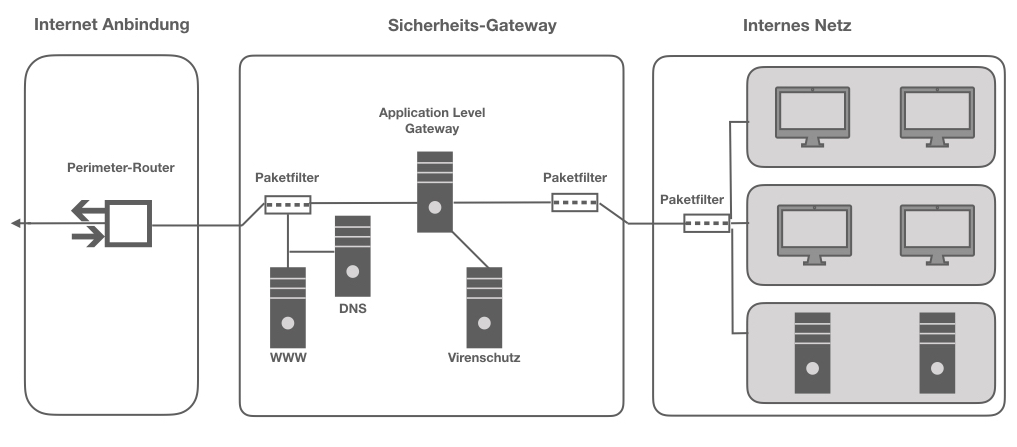
\includegraphics[width=\linewidth]{grundarchitektur}
	\caption{Grundarchitektur eines sicheren Netzwerkes}
	\label{grundarch}
\end{figure}


Die zweite Zone, das Sicherheitsgateway, trennt die InternetAnbindung vom internen Firmennetz. Hier wird eine P-A-P Struktur empfohlen, bestehend aus einem Paketfilter auf der Seite des lokalen Netzes, sowie einem Paketfilter auf Seite des Internets, die jeweils die Kommunikation auf der dritten Schicht des Protokollstapel (\ref{A1}), der Vermittlungsschicht oder auch IP-Schicht, filter. Untersucht werden die Headerinformationen der Vermittlungs- und der Transportschicht und die Datenpakete auf dieser Grundlage entweder verworfen oder durchgelassen  \cite{isi-lana}.
 Der Paketfilter auf Seiten des LANs untersucht die nach außen gerichteten Pakete, der Paketfilter auf Seiten der Internetanbindung filtert die aus dem WWW ankommenden IP-Pakete. Zwischen den Paketfiltern wird das \emph{Application-Level-Gateway} angeschlossen. Hierbei handelt es sich um einen Proxy-Server Über den alle Anfragen in das und aus dem Internet laufen. Er tritt als Stelvertreter auf und verschleiert so die Identitäten der  Clients im LAN \cite{zisler2018computer}, seine Aufgabe ist es außerdem die Kommunikation auf Anwendungsebene zu durchleuchten. Er agiert also auf einer höhreren Schicht als die Paketfilter. 
 Der Bereich zwischen den beiden Paketfiltern des Sicherheits-Gateways nennt sich \emph{Demilitarisierte Zone (DMZ)}, hier sollten Dienste untergebracht werden die vom Internet aus erreichbar sein müssen, wie zum Beispiel Web-Server des Unternehmens. 
 
Diese dei Zonen können um die Management-Zone ergänzt werden, von der aus die Administration der Komponenten erfolgt.
\begin{figure}
	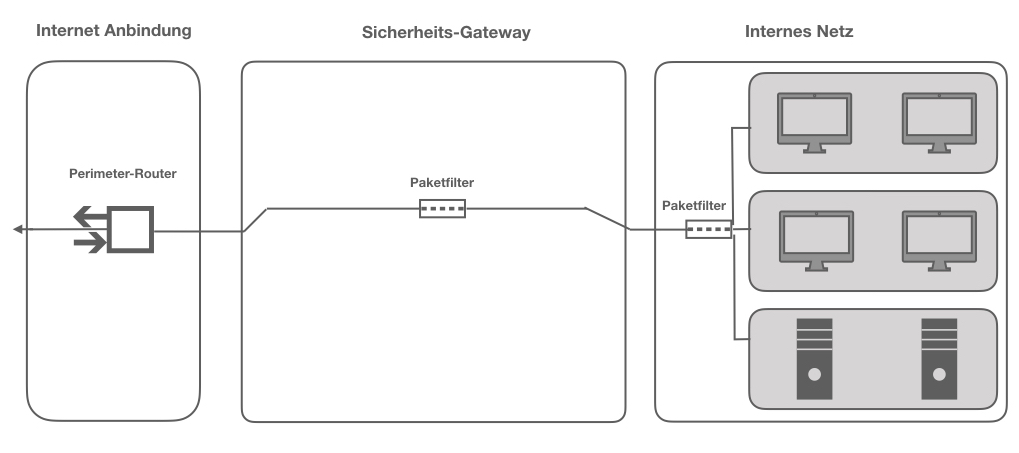
\includegraphics[width=\linewidth]{klUnternHoch.jpeg}
	\caption{Grundarchitektur für ein kleines Unternehmen mit normalem Schutzbedarf}
	\label{klUnorm}
\end{figure}

\begin{figure}
	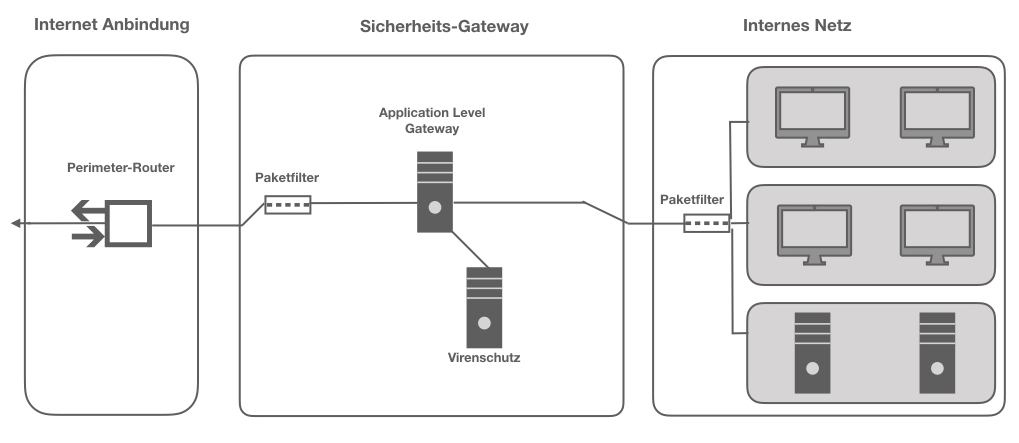
\includegraphics[width= \linewidth]{klUnternehmnorm}
	\caption{Grundarchitektur für ein kleines Unternehmen mit hohem Schutzbedarf}
	\label{klUhoch}
\end{figure}

Aus Kostengründen ist es für kleine Unternehmen oft nicht möglich ein Sicherheitsgateway mit P-A-P Struktur zu betreiben. Für Unternehmen mit normalen Schutzbedarf ist es daher ausreichend, wenn das Sicherheits-Gateway, wie in Abbildung \ref{klUnorm} skizziert, aus einem Paketfilter besteht. 

Für kleine Unternehmen mit hohem Schutzbedarf sollte neben dem Paketfilter auch ein ALG mit Virenschutz betrieben werden. 



